
\section{Boyle's Law}

Name \rule{2.0in}{0.1pt}\hfill{}Section \rule{1.0in}{0.1pt}\hfill{}Date
\rule{1.0in}{0.1pt}

\textbf{Objective}

%test comment

To investigate the relationship between the pressure and volume of
a gas.

\textbf{Apparatus}

\begin{itemize}
\item DataStudio 750 Interface
\item Pasco Pressure Sensor
\item Syringe
\item Tubing
\end{itemize}
\vspace{0.3cm}
{\par\centering 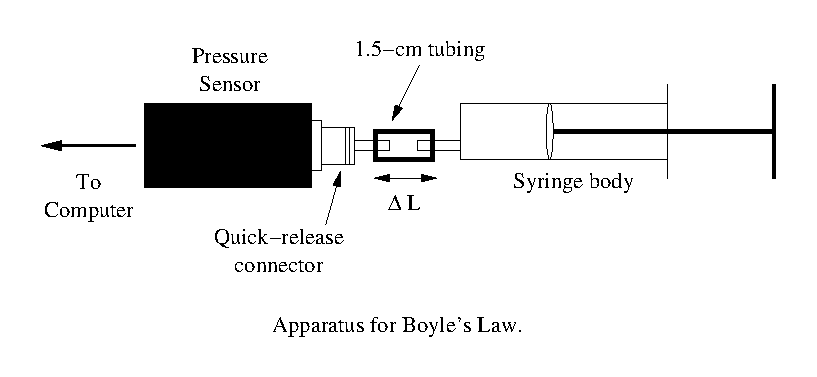
\includegraphics{boyles_law/boyleslawfig1.eps} \par}
\vspace{0.3cm}

\textbf{Introduction}

The behavior of a gas can be described in terms of the macroscopic quantities:
temperature (T), pressure (P), and volume (V). The relationship between these
quantities is given by the equation of state of the gas. A real gas behaves
approximately as an ideal gas if it is far from liquefaction. In that case,
the equation of state of an ideal gas can be used to describe a real gas. For
a given mass of a gas, if one of the quantities P, T, or V is changed, a change
in the other two quantities probably will result. However, if one of the quantities
is kept constant, the relationship between the other two can be studied. The
relationship between pressure and volume of an ideal gas is called Boyle's law.

The experimental apparatus is shown in the figure above. The gas is air contained
in a syringe that has marking on its side to measure the volume of the syringe.
A short tube connects the syringe with a pressure sensor that measures the pressure
in the tube and converts that measurement into a signal that can be read by
the DataStudio interface.

\textbf{Activity 1: Relationship Between P and V of a Gas}

(a) Check that there are no leaks in the apparatus by trying to compressing
the syringe from the 20.0 ml position to the 10.0 ml position. It should become
increasingly difficult to push the plunger as the volume decreases. If this
is not the case, check the couplings for fit. If no problem is obvious, then
consult your instructor. 
\vspace{20mm}

(b) The initial volume of air in the syringe should be set at 20.0 ml. If your
syringe is set to some other value, disconnect the quick release connector from
the sensor by gently rotating it in the counter-clockwise direction as you look
from the syringe toward the pressure sensor. Next, move the piston to the 20.0
ml position, and then re-connect the quick release connector to the pressure
sensor. 

(c) \textbf{Data Recording}. Open the Boyle's Law activity located in the 132
Workshop Folder under the {\bf Start} menu. Click on the window labeled \textit{Volume
and Pressure Table}. This is where your data will be displayed as you record
it. This table display will show the values of the gas volume in the syringe
which you will set by moving the piston to the appropriate marking on the syringe.
You will record the pressure at each of these settings with the pressure sensor.
To begin recording data, make sure the piston is at the 20-ml setting, and click
the Start button. The Start button will change to a Keep button and the table
display will show the value of the pressure next to the first volume value (20
ml) in the table. The reading in the pressure column should be colored red.
Click the Keep button to record this pressure (notice the reading in the Pressure
column beside the 20-ml entry changes from red to black). The next setting for
the volume (18 ml) will appear in the Volume column of the data table display.

NOTE: For the first pressure reading at 20 ml, the air in the syringe will be
in thermal equilibrium with the environment. This will not be the case immediately
after compressing the syringe for the next reading. Therefore, you must allow
a couple of seconds for the system to return to thermal equilibrium after you 
compress the syringe and before clicking on Keep to record pressure values. 

(d) Compress the syringe to the next value of the volume as listed in the data
display table (i.e., the window labeled \textit{Volume and Pressure Table})
and wait a couple of seconds for the system to reach thermal equilibrium. Once 
thermal equilibrium is reached, click Keep to record the pressure. The data 
table display will automatically change to show the next value of the volume 
at which the pressure will be measured. 

(e) Repeat step (d) for the remaining values of the volume listed in the table
display. In other words, continue taking pressure measurements at the prescribed
volume values in the data table display by moving the piston to the prescribed
value and clicking on Keep after thermal equilibrium is reached. After you record
the pressure for the last volume (8 ml), click the small, red box next to the
Keep button (this is the stop button) to end data recording.

(f) \textbf{Analysis.} What happened to the pressure when the volume was 
reduced from 20 ml to 8 ml? From looking at the data, do the pressure and 
volume seem to be directly or inversely proportional? Explain.
%Click on the GraphDisplay to examine the plots of Syringe
%Volume Reading vs. Pressure, and the Volume to Pressure ratio (as a function
%of measuring time). Print the GraphDisplay and attach it to this unit.
\vspace{25mm}

(g) Copy your data into a spreadsheet and plot pressure versus volume 
(including a title and axis labels with units). Next, fit your data with a 
trendline using a power function. Record the result here. What is the power of 
V? Print the graph and include it with this unit.
%What should you get for the power? Why?
\vspace{25mm}

(h) If pressure and volume are inversely proportional, then what can you say
about the product of pressure and volume? Explain.
\vspace{25mm}

\newpage

(i) The measurements you have made are V in milliliters (ml) and P in 
kilopascals (kPa). What are the corresponding units of PV? Show how you get 
this here (the result must be in energy units):
\vspace{40mm}

(j) Construct a table in the space below with the column headings: V (ml), P
(kPa), and PV. Include the units from above in the last column.
Enter the results for P and V in this new table and calculate
PV for each set of readings. Determine the mean value and the standard deviation
\( \sigma  \) for PV. Record the results in the form 
PV = Mean \( \pm \, \sigma  \). Be sure to include the proper units. 
What does this result tell you about the  product PV?

\vspace{12cm}

(k) Is there a trend in the values of PV as the volume decreases? If so, 
what do you suppose causes that trend?

%(j) Examine the plot on the next page with results from two different data 
%runs. How do you explain the difference between the curves for the different 
%tubing lengths (\( \triangle L \) in the diagram on the next page)?

%\vspace{40mm}

%\eject

%\vspace{0.3cm}
%{\par\centering \includegraphics[width=6in]{boyles_law/PVfor132.eps} \par}
%\vspace{0.3cm}

%{\par\centering Results of measurement with Boyle's Law apparatus \par}

%{\par\centering different values of \( \triangle L \), the tubing length.\par}

